 %!TEX root = jsba_main.tex
% Method section

\section{Methods}
\label{sec:meth}
 
 \begin{enumerate}
     \item show how your choice of design and research method is suited to answering your research question(s)
     \item demonstrate that you have given due consideration to the validity and reliability of your chosen method
     \item by “showing” instead of “telling”, you demonstrate that you have understood the practical meaning of these concepts
     \item Show the reader what you have done in your study, and explain why. 
     \begin{enumerate}
         \item How did you collect the data? 
         \item Which options became available through your chosen approach?
         \item What were your working conditions? 
         \item What considerations did you have to balance?
     \end{enumerate}
    \item Tell the reader what you did to increase the validity of your research. 
    \begin{enumerate}
        \item E.g., what can you say about the reliability in data collection? 
        \item How do you know that you have actually investigated what you intended to investigate? 
        \item What conclusions can be drawn on this basis? 
        \item Which conclusions are certain and which are more tentative?
        \item Can your results be applied in other areas? Can you generalise? If so, why? If not, why not?
    \end{enumerate}
    \item You should aim to describe weaknesses as well as strengths. An excellent thesis distinguishes itself by defending – and at the same time criticising – the choices made.
 \end{enumerate}
 
\todo[inline]{Maybe switch following section to implementation chapter instead of methdods}
\todo[inline]{Summarize content of this section briefly}

\subsection{Apache Ignite}
\label{sec:meth_ign}

\citetalias{Ignite} is desribed as a "memory-centric distributed database, caching, and processing platform for transactional, analytical, and streaming
workloads delivering in-memory speeds at petabyte scale" (\citetalias{Ignite}, see also \url{https://apacheignite.readme.io/docs} for the full
documentation).
Its main features are distributed in-memory storage as well as optionally persistent storage of data on the disk that can be treated as a distributed, join
supporting SQL database or as a distributed key-value in-memory data grid. There are a lot more features provided by \citetalias{Ignite} that are not of
relevance here and will be left out because of that reason, thus, in the following there will be a focus on the distributed SQL database part.
Furthermore, the implementation will be based on a pure in-memory storage where all the data will be stored entirely in the RAM without any persistent 
storage of the data due to performance issues. The of \citetalias{Ignite} provided SQL-capable in-memory DDB instances can be spread across the network 
via a set of interconnected Ignite nodes that form a so-called \emph{cluster}. Each node of the cluster can be hosted by a different physical machine 
in a Java Virtual Machine (JVM), but there can be multiple nodes on the same machine, too. Even multiple nodes running in the same virtual machine are
possible. With the underlying Client-Server architecture, a node can be either a server node, which is responsible for storing and processing data, or a
client node that is able to connect remotely to the cluster of server nodes and compute or query from the client side. Figure~\ref{fig:ign_cluster} shows
a sample cluster consisting of 6 server nodes which are responsible for computations and storing data. This servers can be accessed remotely from clients
that can connect to the cluster via an programming language API (e.g. Java), via a JDBC or ODBC connection or via a REST-API (see documentation for
details). 

\begin{figure}[h]
    \centering
    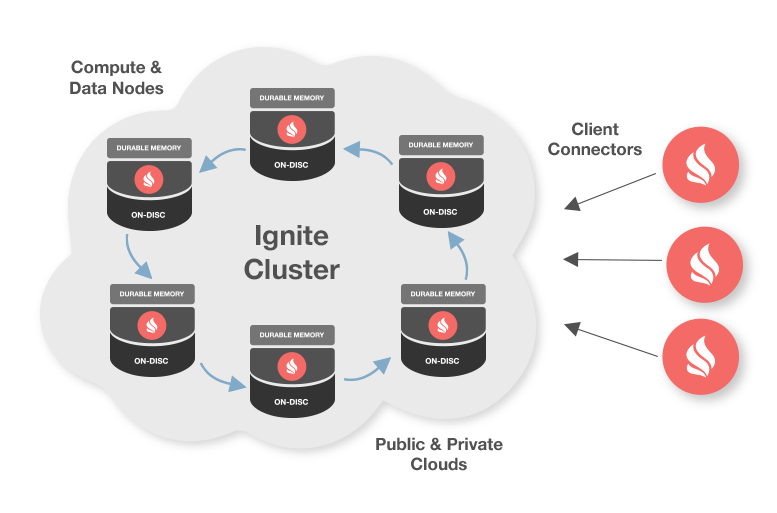
\includegraphics[width=0.75\textwidth,keepaspectratio=true]{img/9287d3c-ignite-deploy.png}
    \caption{Ignite Cluster. Source: \protect\url{https://apacheignite.readme.io/docs/clustering} (Accessed 16th Feb 2019)}
    \label{fig:ign_cluster}
\end{figure}


\subsubsection{Partitioning and Replication}
\label{sec:meth_ign_panre}
The server nodes of an Ignite cluster store some certain data of the whole data set depending on the fragmentation (partitioning, cf.
Section~\ref{sec:theo_ddb_frag}) and replication (cf. Section~\ref{sec:theo_ddb_repl}). The fragmentation and replication is always defined for relations,
i.e. the tables of the relational DDB. For example, under full replication each server would store the total data of the relation and in the partitioned 
mode the relation is partitioned and each server is then responsible for only a subset of the data. It is also possible to have partitioning and 
replication at the same time if the partitions of the data are stored on more than one server such that each partition of the data is stored on one 
server as primary partition and on the other servers as backup copies for higher availability and data resiliency in case of server node failures. 
In replicated mode, a balancing of the data load is achieved by a partitioning of the data of the relation with hash functions into subsets of nearly 
equal size that are dispersed equally among all nodes of the cluster to exploit as much memory as possible on all nodes. However, even more memory is
available if there is no replication of the data in form of redundant copies that would consume additional parts of the total available memory. 

The partitioning is always a horizontal fragmentation of the data but the way how this is computed is only syntactically defined with hash functions, thus,
there are no explicit selection conditions on a certain attribute of the relation that represent a horizontal fragment as described in the
Section~\ref{sec:theo_ddb_frag}, and the assignment of tuples to the partitions of the relation they belong to is done rather arbitrarily. The only way to
influence and change this assignment of a tuple to a partition is via an affinity function, which is explained in the following section.



\subsubsection{Affinity Collocation and Distributed Joins}
\label{sec:meth_ign_affc}

One important concept of \citetalias{Ignite} is the collocation of data with data that corresponds to the concept of a derived horizontal fragmentation 
(cf. Section~\ref{sec:theo_ddb_frag}). Hereby, data that is accessed together, e.g. because it is joined via a common attribute or a foreign key reference,
is also stored together on the same server which improves the data locality~\citep{Wiese2014} and allows for collocated distributed joins that benefit from
this improvement in the data locality as the costly data transfer of data, which is required to obtain an answer to a query, across the network is 
avoided. This \emph{affinity collocation} is internally defined for the key-value store underlying the relational SQL database ensuring that all entries 
of collocated tables where the affinity keys match are stored on the same server. The usage is restricted to a single affinity key definition per 
relation. With this restriction, there can not be a collocation of three or more relations that could be joined via a chain of join conditions where the
joining attributes, that would form a possible affinity key, are different. An affinity key can be the same as the primary key of the relation or an 
attribute of a composite primary key of the relation. The concept of affinity collocation strongly corresponds to the primary and derived horizontal
fragmentation of relations (cf. Section~\ref{sec:theo_ddb_frag}), i.e. the derived fragmentation also ensures that tuples from the derived horizontal 
fragments are located at the same server where also the tuples reside with which they can and will be joined in SQL queries.

Joins between partitioned relations require for collocation of the data that is about to be joined. Otherwise, a non-collocated distributed join has to be
performed or the result set will be incomplete as the non-collocated parts of the data can not be joined locally by the nodes. If all the joined relations
in the SQL query are collocated, the query can be evaluated locally by each node, because all the data they need to compute a correct result set regarding 
their portion of the whole data in the cluster is available, i.e. stored by themselves. The query execution for this case is depicted in
Figure~\ref{fig:ign_collocated} where the query $Q$ is sent from the client to each server node which executes the query $Q$ locally 
and returns the result set $R_i$ to the query according to its stored data set. The final result set is the accumulation of the result sets $R_1+R_2+R_3$
which is meant as union of the result sets. This computation of the result set as union of locally obtained result sets is very similar to the localization
program \cite[p.~199]{Ozsu1991} as introduced in Section~\ref{sec:theo_dqp_decomp} where the union of all the fragments of certain relations is used to
rewrite the query in order to execute it in a distributed fashion.  
\begin{figure}[ht]
    \centering
    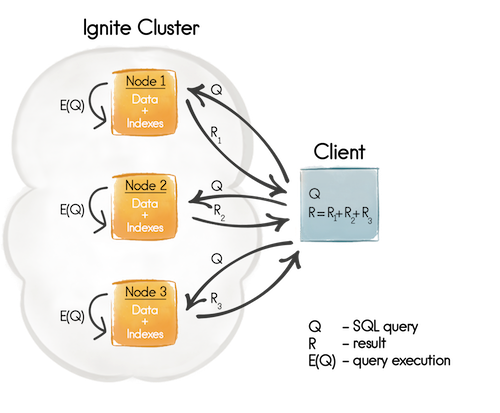
\includegraphics[width=0.6\textwidth,keepaspectratio=true]{img/2af89cf-Collocated_sql_queries.png}
    \caption{Collocated SQL Query. Source: Picture 1, \protect\url{https://apacheignite-sql.readme.io/docs/distributed-joins} (Accessed 16th Feb 2019)}
    \label{fig:ign_collocated}
\end{figure}

On the other side, non-collocated joins require for additional communication and data transfer between the nodes of the cluster as the data, that is needed
for a join or another computation, is not locally present, thus, the nodes have to sent requests for the data to other nodes to complete their result set 
computations appropriately. This additional data transfer implies a bad efficiency of query execution as it depends on the transmission duration of
probably bigger data sets between the nodes. Furthermore, this causes additional load on the network that can decrease the performance of other tasks or
operations. Non-collocated joins must be enabled explicitly in \citetalias{Ignite} to enforce the distributed answering with data transfer across the
cluster if necessary. If not enabled explicitly, the query will be executed in a collocated manner which, in general, leads to incomplete result sets due
to the unavailable locality of required data. The general flow of a query execution of a non-collocated, distributed query is sketched in
Figure~\ref{fig:ign_noncoll}. 
\begin{figure}[ht]
    \centering
    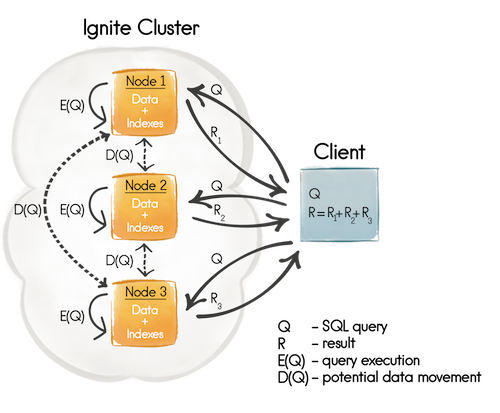
\includegraphics[width=0.6\textwidth,keepaspectratio=true]{img/95f09db-Non_collocated_sql_queries.png}
    \caption{Non-Collocated SQL Query. Source: Picture 2, \protect\url{https://apacheignite-sql.readme.io/docs/distributed-joins} (Accessed 16th Feb 2019)}
    \label{fig:ign_noncoll}
\end{figure}
 
In comparison to Figure~\ref{fig:ign_collocated}, the additional data transfer, that might occur in relation to the non-collocated query, is depicted as
potential data movement $D(Q)$ in a peer-to-peer fashion between all pairs of nodes. However, the data request of a node can be sent as a unicast request 
to a certain node of the cluster (peer-to-peer communication) or as a broadcast request to all other nodes. This decision depends on whether the 
requesting node can identify the exact location of the data, i.e. if it is a join on a primary or affinity key, or if it has to request the missing data
from all other nodes otherwise. 

 
 
\subsection{Clustering-based Fragmentation}
\label{sec:meth_cbfr}

The \emph{clustering-based fragmentation} \citep{Wiese2014} is a horizontal fragmentation strategy that, on the one hand, enables fragmentation regarding 
a similarity metric which allows for a more semantic partitioning of the data set, and, on the other hand, supports the \emph{similarity-based query
answering} (cf. Section~\ref{sec:meth_sbqa}), and the, for example in case of a query failure, desired \emph{flexible query answering} 
(cf. Section~\ref{sec:meth_fqa}). The underlying clustering is computed based on an approximation algorithm \citep{Gonzales1985} with respect to all 
values that can occur for a chosen \emph{relaxation attribute} of the relation, the \emph{active domain} as defined in the following (according to
Definition 2 in \cite{Wiese2014}). The pseudocode of the clustering procedure is described in Listing~2 in \cite{Wiese2014}.

\begin{definition}
Given a relaxation attribute $A$ and a relation instance $R$ (set of tuples), let $\pi_A(R)$ denote the \emph{active domain} of the relaxation attribute
$A$ of the relation $R$.
\end{definition}

With the chosen relaxation attribute $A$ of a relation $R$ and a pairwise similarity $sim(a, b)$, $\pi_A(R) \times \pi_A(R) \to \mathbb{R}$, defined  
for pairs of elements from the active domain $\pi_A(R)$ and according to the formal mathmatical definition of a metric, a clustering in terms of a 
partitioning of the active domain into disjunctive subsets can be obtained by evaluating the similarities and assigning the elements to the clusters in
a such way that the pairwise intracluster similarity is always at least as big as the pairwise intercluster similarity. This means that any element has 
a higher similarity to elements of the same cluster than compared to elements from other clusters, thus, a cluster describes rather similar elements. 
An appropriate criterion for determining how "similar" two elements have to be to belong to the same cluster is required and can be defined as a threshold
parameter $\alpha$ and a \emph{head} element representing the cluster that enforce a minimal intracluster similarity \cite{Gonzales1985}. Under this
restriction, for any element $a$ of a cluster, the corresponding $head$ element of this cluster and a given threshold $\alpha$ holds that 
$sim(a,head) \geq \alpha$. 


The different clusters contained in the clustering can be used to obtain a horizontal fragmentation of a relation by partitioning the relation along the 
disjunctive subsets of elements from the active domain with respect to the relaxation attribute. Each cluster corresponds to one horizontal fragment where
the tuples are mapped to a fragment based on the membership of the relaxation attribute's value in the tuple to the subset of elements in a cluster. This 
can be defined as follows (cf. \cite[Definition~2]{Wiese2014}):

\begin{definition} \label{def:cbfr}
Given the active domain $\pi_A(R)$ regarding a relaxation attribute $A$ of a relation instance $R$, and a complete clustering $C=\{c_i|i=1,...,n\}$
of $\pi_A(R)$ with threshold $\alpha$ and head elements $head_i \in c_i$ for the clustering. Then, $F=\{R_1,...,R_n\}$ is a (horizontal) 
\emph{clustering-based fragmentation} of $R$ if
\begin{itemize}
    \item every horizontal fragment $F_i$ corresponds to one cluster $c_i \in C$ such that $c_i=\pi_A(F_i)$
    \item $\forall i \in \{1,...,n\}: \forall a \in c_i: sim(a, head_i)>=\alpha$
    \item the fragmentation $F$ is correct (\cite[p.~103]{Ozsu1991})
\end{itemize}
\end{definition}

The completeness for the clustering, that is required in Definition~\ref{def:cbfr} and in Definition~2 in \cite{Wiese2014},
provides coverage for all elements of the active domain $\pi_A(R)$ regarding the relaxation attribute $A$. Furthermore, the mapping of any element of the
active domain to one of the clusters is functional which makes the clusters pairwise disjoint, hence, all the by the clustering induced fragments are also
disjoint and non-redundant as each tuple is assigned to only fragment according to its relaxation attribute's maximum similarity to one of the clusters.
Thus, the relation instance $R$ can be reconstructed from the horizontal fragments with its localization program. Covering these three aspects, the
obtained fragmentation is a correct fragmentation \cite[p.~103]{Ozsu1991}. The following example illustrates the clustering-based fragmentation without
concerning a concrete similarity in terms of a metric but with a intuitive idea of similarity. The behavior of the clustering procedure when scaling the
threshold parameter is analyzed in Section. \todo[inline]{Ref alpha scaling}

\begin{exmp}
\label{sec:meth_cbfr_exmp}
Consider the clustering $C=\{c_1, c_2, c_3\}$ with three clusters $c_1$,$c_2$ and $c_3$, where $c_1=\{"Car","Bus","Truck"\}$, 
$c_2=\{"Ferry","Row~boat","Speedboat"\}$ and $c_3=\{"Airplane","Glider","Helicopter"\}$. The clustering obviously clusters a set of vehicle describing 
terms according to the categories of their area of usage, which are land, sea and air, respectively. The clustering indicates that different aircrafts 
are more similar than for example a boat and an airplane are. In addition to this clustering, consider the relation $Products$ with the relaxation
attribute $Category$ as shown in Table~\ref{tab:cbfr_products}.

\begin{table}[h]
    \centering
    \begin{tabular}{|c|c|c|}
        \hline
        Name & Category & Price \\
        \hline
        XFast & Car & 50.000€ \\
        Rowy & Row boat & 999€ \\
        UFO-9 & Airplane & 100.000.000€ \\
        \vdots & \vdots & \vdots \\
        \hline
    \end{tabular}
    \caption{Relation $Products$ describing different vehicles that are sold by a company}
    \label{tab:cbfr_products}
\end{table}

The clustering-based, horizontal fragmentation of the relation $Products$ consists of three fragments, $F_1$, $F_2$ and $F_3$, where fragment $F_i$
includes all the tuples from the relation $Products$ that are categorized by a term that belongs to the cluster $c_i$ (cf. Definition~\ref{def:cbfr}), 
i.e. the first fragment contains the tuple of the car named "XFast", the second fragment contains the tuple of the row boat named "Rowy", etc., as
illustrated by Table~\ref{tab:cbfr_frags}.

\begin{table}[h]
    \hspace*{\fill}
    \begin{tabular}{|c|c|c|}
        \hline
        Name & Cat. & Price \\
        \hline
        XFast & Car & 50k€ \\
        \vdots & \vdots & \vdots \\
        \hline
    \end{tabular}
    \hfill
    \begin{tabular}{|c|c|c|}
        \hline
        Name & Cat. & Price\\
        \hline
        Rowy & Row boat & 999€ \\
        \vdots & \vdots & \vdots \\
        \hline
    \end{tabular}
    \hfill
    \begin{tabular}{|c|c|c|}
        \hline
        Name & Cat. & Price\\
        \hline
        UFO-9 & Airplane & 100M€ \\
        \vdots & \vdots & \vdots \\
        \hline
    \end{tabular}
    \hspace*{\fill}
    \caption{Clustering-based, horizontal fragments fragments $F_1$, $F_2$ and $F_3$ (from left to right) of relation $Products$ 
            (Table~\ref{tab:cbfr_products})}
    \label{tab:cbfr_frags}
\end{table}

\end{exmp}

As the clustering-based fragmentation is a primary horizontal fragmentation, it is also possible and efficient to derive another horizontal fragmentation
from it in the same way as already discussed in Section~\ref{sec:theo_ddb_frag}. This is the collocation of the data that first of all assigns all tuples
of the primary relation to fragments according to the cluster (cf. Example~\ref{sec:meth_cbfr_exmp}), and then collocates tuples of the other relations to
the corresponding derived, horizontal fragments.


\subsection{Similarity-based Query Answering}
\label{sec:meth_sbqa}

A DDBS that uses a clustering-based fragmentation and derived fragmentations -- as described above -- is capable of answering queries regarding the 
similarity defined for the relaxation attribute underlying the clustering. This means that, for certain queries, the system is able to utilize the 
similarity metric in order to determine the relevant fragments to obtain an answer to the given query. As the data is distributed along the clustering to
the horizontal fragments of the fragmented relation, the query execution can also be distributed according to the clustering to be executed as close as
possible to the location of the data, i.e. in the best case it is sufficient to execute the query only locally without any data transfer at a single 
server which hosts the single relevant data fragment. Finding the appropriate fragment depends on whether the query contains at least one selection
condition on the relaxation attribute of the clustering. If so, the corresponding fragment can be identified by evaluating the similarity of the element
from the active domain, to which the relaxation attribute is compared, to the head elements of the different clusters. The maximal similarity of the 
comparison element and all cluster heads determines the matching cluster as well as the induced horizontal fragment. 

\begin{exmp}
\label{sec:meth_sbqa_exmp}
Consider again the clustering-based fragmentation of the relation $Products$ as introduced in Example~\ref{sec:meth_cbfr_exmp} and an assignment of the 
fragments $F_1$, $F_2$ and $F_3$ to three different servers, $S_1$, $S_2$ and $S_3$, respectively (cf. Table~\ref{tab:cbfr_frags}). Assume that a potential
customer of the company is interested in purchasing an airplane and queries the database, for instance via an interface on the web page of the company, 
for all vehicles matching his interest. The query could be
\begin{verbatim}
    SELECT Name, Price FROM Products WHERE Category = 'Airplane'
\end{verbatim}
and could be answered in an efficient way by using similarity-based query answering to restrict the query execution such that the query is only sent to 
one server which is responsible for the aircraft-vehicles-fragment of the $Products$ relation and executed locally on this server. Hence, only server 
$S_3$

Without this optimization, the query would have to be processed and executed by all servers that store a fragment of the $Products$ relation. However, 
all servers except the server hosting the required fragment will return an empty answer as they have no matching tuples in any of their fragments. But 
this still means that even if there are no matching tuples at a server because it does not host the relevant fragment, the pure query answering, i.e.
without an intelligent, similiarity-based answering and optimization, entails that all tuples of fragments of the relation $Products$ have to be checked.
As scanning all potential answer tuples obviously scales with the size of the relation and the fragments, the execution of the query will be less 
efficient when the data set grows big.
\end{exmp}

\todo[inline]{Maybe some more content here...?}


\subsection{Flexible Query Answering}
\label{sec:meth_fqa}

As already mentioned in the introduction, failing queries, that have an empty result set, are only desirable for a user in the fewest cases as an empty
result cannot provide any information except the information that this certain query could not be answered exactly under the current database state. For
example, consider a database that stores logs of a running application in different relations according to common log levels, e.g. "WARN", "INFO" and
"ERROR". If a query asking for all the logs that are labelled as errors is stated against this log database, an empty result would be satisfying, for 
instance, for a software engineer, who is involved in the development or maintenance of the application, as the information induced by the empty answer 
means that no unwanted errors occurred. But in most of the cases, a failing query forces the user to check whether the query contains some logical error
itself leading to no exact answers, or whether the current database state does actually not provide any matching data. Both of the points are not always
easy to check as the initially stated query can be really complex. Nevertheless, in case of the second criterion, the database would probably be able to
give an answer that has an informational content that is \emph{similar} to an exact answer and, in contrast to the exact answer, non-empty. Therefore, the
user could already be satisfied with a similar answer as this similarity can already enable the user to gain information and draw conclusions based on this
similar answer.
\todo[inline]{Maybe again highmed oncology use case}
\todo[inline]{Generalization, Anti-Instantiation, etc.}

\subsubsection{Query Generalization}
In general, queries can be answered flexibly by \emph{deductive generalization} \citep{Gaasterland1992, Wiese2014} that expresses that in first-order logic
(FOL) a formula $\Psi(X,Y)$ over the free variables contained in vectors $X$ and $Y$, where $X$ and $Y$ contain only different free variables, deductively
generalizes the formula $\Phi(X)$ if for a given knowledge base $\Sigma$ holds that $\Sigma \vDash \forall X \exists Y (\Phi(X) \to \Psi(X,Y))$ 
(cf. Definition~1 in \cite{Wiese2014}). In a special case, a knowledge base can be a relational (distributed) database that describes a logical language by
its relations as the predicate symbols, a domain of all constant symbols which occur in the table columns and a set of variables to express queries 
(cf. \cite{Wiese2014}). For instance, the relation $Products$ from the previous examples would be represented by the predicate symbol $Products(x,y,z)$
and the query from Example~\ref{sec:meth_sbqa_exmp} could be expressed as the logical formula $Q(N,P)=Products(N,P,"Airplane")$, that binds the free 
variables $N$ and $P$ to name and price, respectively, of all tuples in the database that have the category airplane. 

\subsubsection{Anti-Instantiation}
One common generalization operator is the \emph{anti-instantiation} operator \citep{Wiese2014} that deducts a more general formula by substituting a
constant symbol with a variable or by substituting an at least twice occuring variable by a new variable. For example, the query formula $Q(N,P)$ would 
be anti-instantiated by replacing the constant symbol $"Airplane"$ by a new variable $Z$ which results in the more general query
$Q'(N,P,Z)=Products(N,P,Z)$ (or also possibly $Z$ bound by an existential quantifier). Obviously, every variable binding that satisfies the less general
formula $Q(N,P)$ also satisfies the more general one, thus, $Q'(N,P,Z)$ is a deductive generalization of $Q(N,P)$. In terms of SQL, the anti-instantiated
formula is equal to the SQL query 
\begin{verbatim}
   SELECT * FROM Products 
\end{verbatim}
where again every tuple satisfying the less general SQL query also occurs in the result set of the more general query. However, the application of this
generalization operator can cause a so-called \emph{overgeneralization} \citep{Wiese2014} that -- regarding queries and query answering -- results in 
too general answers which are not closely related to the intended answers anymore and so may not be informative at all. This is also indicated by the
just examined query and its generalization which returns all tuples of the relation $Products$ although most of the information about a vehicle is not
similar to the desired information about airplanes. Instead, more semantics can be added in an intelligent combination of deductive generalization in form
of anti-instantiation with the clustering-based fragmentation in order to obtain more general queries that are based on the underlying similarity metric
for the clustering. This can be achieved by replacing a constant symbol from the relaxation attribute's domain by a new free variable that is resricted to
only the values that belong to the same cluster to which the constant symbol belongs to. In FOL this can be expressed by a disjunction that covers all the
possible constant symbols of the cluster, e.g. $Q'(N,P,Z)=Products(N,P,Z) \land (Z="Airplane" \lor Z="Glider" \lor Z="Helicopter")$. This query is also
more general but it contains a more intelligent selection of not all vehicles but only the ones that are similar to airplanes as they can also fly. The
following example also shows how the anti-instantiation can be realized in SQL with an underlying clustering-based fragmentation providing the ability
to answer queries flexible and similarity-based resulting in reasonable and informative answers that are not too general as a semantic guidance 
\citep{Wiese2014} avoids overgeneralization.

\begin{exmp}
\label{sec:meth_fqa_exmp}
Again, let the subject of this example be the relation $Products$ and the underlying clustering-based fragmentation on the relaxation attribute $Category$
as in Examples~\ref{sec:meth_cbfr_exmp} and \ref{sec:meth_sbqa_exmp}. Consider also the situtation where another prospect who this time is interested in 
purchasing a helicopter instead of an airplane states a corresponding query like
\begin{verbatim}
    SELECT Name, Price FROM Products WHERE Category = 'Helicopter'
\end{verbatim}
against the database. This query will fail if the $Products$ relation contains no vehicle tuple which satisfies the condition \verb!Category='Helicopter'!
in the current database state because the company does not produce and sell helicopters currently. With the given clustering of the relaxation attribute,
the query could be rewritten and generalized to provide similar answers based on the similarity of other aircrafts to the initially queried helicopters.
There are multiple ways to rewrite the query to achieve this generalization but all extend the query such that it is fulfilled by all tuples that match the
contained selection condition on the category of the vehicle with any aircraft representing term:

\begin{itemize}
    \item \begin{verbatim}
    SELECT Name, Price
    FROM Products 
    WHERE Category IN ('Helicopter', 'Airplane', 'Glider')
    \end{verbatim}
    
    \item \begin{verbatim}
    SELECT Name, Price 
    FROM Products 
    WHERE Category = 'Helicopter' 
        OR Category = 'Airplane' 
        OR Category = 'Glider'
    \end{verbatim}

    \item \begin{verbatim}
    (SELECT Name, Price FROM Products WHERE Category = 'Helicopter')
    UNION 
    (SELECT Name, Price FROM Products WHERE Category = 'Airplane')
    UNION 
    (SELECT Name, Price FROM Products WHERE Category = 'Glider')
    \end{verbatim}
\end{itemize}

All three queries produce the same result set which, on the contrary, can contain some at least similar information compared to the initially failing,
non-generalized query. Besides this query generalization in order to return all available data about aircrafts, the user's interest to buy an aircraft of
another category which is actually sold might be aroused when getting the information about this similar alternatives which might be beneficial for the
company. 

Indeed, flexible query answering that is based on some semantic guidance, like the clustering based on the similarity defined for disease representing 
MeSH terms, can be really helpful when considering the search for similar patient profiles for decision making regarding the treatment options and for 
predictions for the patient's future (cf. oncology use case in \cite{Haarbrandt2018}). The data of identified similar patients can be used to compare the
current situation of the patient as well as probabilities of success or failure of treatments. The higher the similarity is to other patients, the higher 
is also chance for an optimal treatment of the cancer disease, especially early detection and methods of prevention could be enabled. But as the 
similarity crosses some arbitrary threshold, also the informational content that can be derived and concluded will not be as useful anymore.
However the reliable identification of similar cases, for example for cancer diseases, requires way more complex semantic similarity measures in order 
to identify helpful profiles and information that can not be handled by simple query generalization but allow for ranking similar cases based on the
similarity measures \citep{Haarbrandt2018}.

\end{exmp}